%% by Michael Shell
%% Edited by Dominic Carr
%%
%% This work is distributed under the LaTeX Project Public License (LPPL)
%% ( http://www.latex-project.org/ ) version 1.3, and may be freely used,
%% distributed and modified. A copy of the LPPL, version 1.3, is included
%% in the base LaTeX documentation of all distributions of LaTeX released
%% 2003/12/01 or later.
%% Retain all contribution notices and credits.

\documentclass[10pt,journal,compsoc]{IEEEtran}

\hyphenation{op-tical net-works semi-conduc-tor}

\usepackage{lipsum} 
\usepackage{hyperref}
\usepackage{biblatex}
\usepackage{graphicx}
\usepackage{listings}
\usepackage{amsmath, xparse}

\graphicspath{{./../images/}}

\addbibresource{test.bib}

\begin{document}
% paper title
% Titles are generally capitalized except for words such as a, an, and, as,
% at, but, by, for, in, nor, of, on, or, the, to and up, which are usually
% not capitalized unless they are the first or last word of the title.
% Linebreaks \\ can be used within to get better formatting as desired.
% Do not put math or special symbols in the title.
\title{Teaching a Neural Network to Fly Autopilot}

% author name
\author{Otito~Mbelu (G00397738)% <-this % stops a space
}

% The paper headers
\markboth{Atlantic Technological University - Artificial Intelligence Assignment}%
{}

\IEEEtitleabstractindextext{
    \begin{abstract}
        The goal of this project is to train a Automatic Neural Network to navigate through 
        an endless horizontally scrolling tunnel without clipping any of the edges. A programmed agent 
        capable of consistently navigating the tunnel accurately was designed and implemented, and was
        further used as a trainer to generate training data for the Neural Network. Model selection 
        was done using a brute force approach that calls for a grid search using varying ranges of 
        hyper parameters to select an optimum model. Metrics for model evaluation was based on 
        F1-Accuracy score and Mean Cross-Entropy Loss through cross-validation with training data.
        A network configuration of 21-20-3 with Rectified Linear Unit Activation Function 
        (RELU) with a test accuracy score of 100\% and MCCE loss of 0.1839 was selected as the best 
        model. Furthermore, an autopilot agent utilizing Fuzzy Logic was implemented to solve the 
        problem. 

    \end{abstract}
}

% make the title area
\maketitle

\section{Introduction}
\label{sec:introduction}

\IEEEPARstart{T}{}he game consists
of a 30 $\times$ 20 grid where the ship is at a fixed column and can navigate vertically i.e. up and 
down. A programmed agent capable of flawlessly navigating the tunnel in a consistent manner was designed
to be the basis of training data generation. The agent's navigation algorithm was designed in the basis 
of navigating the ship through the middle of the weighted opening in the next $n$ columns with respect to 
the ship current location. This implies that the next movement of the ship will attempt to get closer to 
the weighted center of the next $n$ columns. A look forward horizon of $3$ was chosen as the value for $n$.
After trials with the ranges $2 \to 5, 3$ was selected because it performs the smoothest navigation through
the tunnel amongst the values trialed. This resulted in a grid of $n \times (2n + 1)$ i.e. $3 \times 7 = 21$ 
input features. The following sections describes the design and model selection strategy used to implement
the various agents. 

\section{Agent Design}
All the AutoPilot agents implements the base abstract class Agent, which provides all the functionality for 
sampling and preprocessing data. 


\subsection{Programmed Agent}

The behavior of this agent was implemented on the $ProgrammedAgent$ class. To predict which step to take, the
weighted center of the opening of the cave is evaluated for a given horizon $n$ using the softmax function 
of the proximity as weights. $W = \sigma(N)$,
where $\sigma$ is the softmax function and $W$ is weight, $W = \{w_1, w_2, ..., w_n\}$ and $N = \{1, 2, ..., 
n\}$. The weighted center is evaluated by taking the mean of the dot product of the weight and 
the center of each column (See Fig.~\ref{fig:stage}). $y = \frac{1}{n}\sum\limits_{i=1}^{n}W_i \times \frac{h_i}{2} = \frac{1}{2n}
(W \cdot H)$ where $h_i$ is the height of the cave's opening for column $i$ and $H$ is the set of heights. 
The final prediction is determined by the value of $y$ with 
respect to the ships current row. The ship will navigate UP if $y > player\_row$ and DOWN if $y 
< player\_row$ and will STAY put if $y = player\_row$



\section{Sampling}
\subsubsection*{Buffering}
Data sampling strategy involves storing the entire grid beyond the ship's location (column) in a buffer and 
continuously consume the buffer until it runs out. The buffer will be refilled as soon as the buffer is 
exhausted. A pointer which points to the current position in the buffer was used to track the position of 
the buffer. The size of the buffer is given by $b_w \times b_h$, where $b_h$ is the height of the stage and 
$b_w$ starts from column next to the ship to the very end of the stage on the horizontal axis. 
This is demonstrated in Fig. \ref{fig:sampling}. This implies that new data is sampled every
$b_w - n$ frames, where $b_w$ is the width of the buffer and $n$ is the horizon. 
\subsubsection*{Feature Extraction} 
At any given frame the agent will have to extract the relevant features from the buffer which is the next $n$
columns beyond the ship (see Fig.\ref{fig:sampling}) with a height of $2n + 1$. The relevant features is given
as $F = \bigcup\limits_{i=1}^{n}F_i$, where $F_i$ is the $i$th column of the relevant features and the union 
operation represents arraycopy. $F_i = \bigcup\limits_{j = p(b_h) + r - n}^{2n + 1} B_j$, where $p$ = pointer,
 $r$ is player row, $b_h$ is the height of the buffer and $B_j$ is the $j$th column of the 
buffer $B$. Data extraction runs at a big O of $O(|F|)$ where $|F|=n \times (2n+1)$, assuming that arraycopy
is done at $O(1)$.


\section{Feature Design}

The value 3 was chosen for $n$ i.e. the horizon, which resulted in 21 input features for the Neural Network. 
A classification model was chosen as three different output is expected, thus the output of the Neural 
Network consists of 3 nodes.
 
The selected input features for the model does not include the position of the ship. This decision was made 
after analyzing the training data which showed that the one-hot encoded values for the position only varies
in 2 out of 630 training dataset. And thus was considered redundant.

\section{Model Selection}
A grid search algorithm taking different values for $\alpha, \beta$, epochs, activation functions, loss 
functions, training speed, number of nodes per layer, number of hidden layers was implemented and used
to search for the best model. The following range of values were used for the grid search, $\alpha \to (0.01, 0.001,
0.0001)$, $\beta \to (0.5, 0.75, 0.95)$, $min\_error \to (0.0001, 0.00001)$, $epochs \to (300, 500)$, 
$loss\_functions \to (CEE, MSE, SSE)$, $act\_functions \to (TANH, RELU, ISRLU)$, $layers \to (1, 2)$
Table~\ref{table:top_models} shows a summary of different models selected and their 
respective performances. 

\subsubsection*{Metrics}
Cross validation of 5 fold was used for model evaluation, and final performance recorded with unseen test
data. F1-Accuracy was used as the first benchmark for model selection while the cross entropy loss was 
used as a tie breaker for models with similar F1-Accuracy scores. 

\subsubsection*{Best Model}
The best model was selected after evaluating all the models using unseen test data and the overall best performant
model recorded a test accuracy of 100\% and Mean Categorical Cross Entropy Error of 0.1839.
The hyper-parameters and configuration for the best model are listed as follows:
$\alpha = 0.01,\beta = 0.75, loss=CEE, max\_epochs = 300$, hidden layers = 1, topology = 21-20-3. 


\section{Extra - FuzzyAgent}
This agent was implemented using a Fuzzy Inference System (FIS). 
\subsubsection*{Fuzzification}
The input variable to FIS is given by $\phi$ and $\psi$. The universe of discourse is given by the  
$\Phi$ and $\Psi$ which both have ranges of
$-90^{\circ} \to 90^{\circ}$. $\phi \in \Phi$, represents the angle of inclination of the ship with respect to the top clip of the cave
opening, while $\psi \in \Psi,$ represents the angle of declination of the ship with respect to the bottom clip
of the cave opening. $\phi$ and $\psi$ were evaluated as the weighted average of the angles between
the ship and the cave's top and bottom edges of the opening along its horizon respectively. $\phi = W \cdot \vec{\phi}, 
\psi = W \cdot \vec{\psi}$, where $\phi = \{\phi_1, \phi_2, ..., \phi_n\}, \psi = \{\psi_1, \psi_2, ..., 
\psi_n\}$ and $\phi_i = tan^{-1} \left(  \frac{y_{t_i}}{x_{t_i}}\right)$ and $\psi_i= tan^{-1} \left(  
\frac{y_{b_i}}{x_{b_i}}\right)$. 
The output of the FIS $f(\phi, \psi)$ were evaluated using the Center Of Gravity (COG) defuzzification 
technique.
\subsubsection*{Membership Function} 
The Membership functions for the input variables were defined by the Linguistic variables $high$ and $low$, and maps $\phi$ and $\psi$ to 
$\mu_{\Phi}$ and $\mu_{\Psi}$ respectively. The output $f(\phi, \psi)$ was defined using the linguistic variable
$up$, $down$, and $still$ (See Fig.\ref{fig:fuzzy})

\subsubsection*{Rules}
The rules for FIS were defined as follows: 
$\footnotesize{\texttt{1 : IF $\phi$ IS low AND $\psi$ IS low THEN output IS down;}}$
$\footnotesize{\texttt{2 : IF $\psi$ IS high AND $\phi$ IS high THEN output IS up;}}$
$\footnotesize{\texttt{3 : IF $\psi$ IS low AND $\phi$ IS high THEN output IS still;}}$
$\footnotesize{\texttt{4 : IF $\phi$ IS low AND $\psi$ IS high THEN output IS still;}}$

\section{Conclusion}

A programmed agent was designed as a training agent and was used to generate training data. 
A total of 1671 Neural Network models using 673 training data was built. 25\% of the training data was reserved for 
testing and 75\% was used for training and validation. Tabulated summaries of the evaluation results are presented 
in the Appendix. Both the NeuralNetwork Agent and FuzzyAgent were successfully implemented to navigate through the cave successfully. 
Buffering was implemented, which significantly reduced the frequency of sampling data. Data processing and evaluation 
libraries were developed to properly evaluate the models.
However, there have been recorded rare instances of the FuzzyAgent clipping the edges of the cave resulting in a crash.


\appendices
\begin{table}[hbt]
    \centering
    \begin{tabular}{|l|l|l|l|l|l|l|l|l|}
    \hline
        Index & Layers & Act. & Loss & Epochs & Alpha & Beta & Acc.\(\%\) & MCE \\ \hline
        1132 & 21-15-20-3 & ISRLU & SSE & 500 & 0.01 & 0.95 & 100.00 & 0.1819 \\ \hline
        1120 & 21-15-20-3 & ISRLU & SSE & 500 & 0.01 & 0.5 & 100.00 & 0.1827 \\ \hline
        1048 & 21-15-20-3 & ISRLU & MSE & 500 & 0.01 & 0.5 & 100.00 & 0.1835 \\ \hline
        1067 & 21-20-45-3 & ISRLU & MSE & 300 & 0.01 & 0.95 & 100.00 & 0.1835 \\ \hline
        1049 & 21-20-45-3 & ISRLU & MSE & 500 & 0.01 & 0.5 & 100.00 & 0.1836 \\ \hline
        30 & 21-12-3 & ISRLU & CEE & 500 & 0.01 & 0.95 & 100.00& 0.1838 \\ \hline
        31 & 21-15-3 & ISRLU & CEE & 500 & 0.01 & 0.95 & 100.00& 0.1838 \\ \hline
        33 & 21-12-3 & ISRLU & CEE & 300 & 0.01 & 0.95 & 100.00& 0.1838 \\ \hline
        240 & 21-12-3 & ISRLU & SSE & 500 & 0.01 & 0.95 & 100.00 & 0.1838 \\ \hline
    \end{tabular}
\end{table}

\begin{figure}
    \centering
    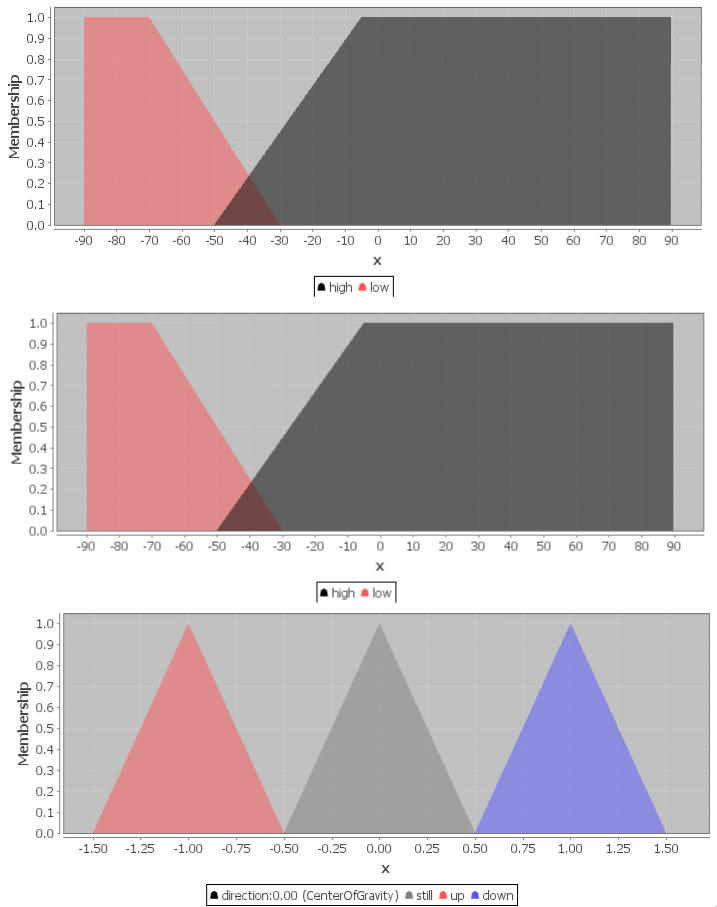
\includegraphics[width=\linewidth]{fzzy.png}
    \caption{Sampling}
    \label{fig:sampling}
\end{figure}
\end{document}